\section{OpenCV}
\label{opencv}

%Intro
OpenCV\cite{opencv} (Open Source Computer Vision) is a library that implements state of the art real-time computer vision 
algorithms. 

It is cross-platform and it is released under a BSD\cite{BSD} license. Previously it was integrated in ROS \cite{ros}, but
now it is used as a stand-alone library.  

\begin{figure}[h]
	\begin{center}
    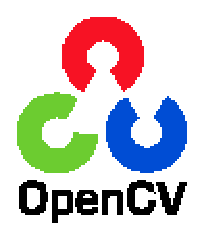
\includegraphics[scale=1]{img/opencv/logo.eps}
	\caption[OpenCV Logo]{OpenCV Logo}
	\end{center}
\end{figure}

The qualities described above as well as its optimization of various algorithms make this library an extremely useful asset for robotic vision projects. 

% In this project's context

In this project the C++ interface of the OpenCV library has been used. The functionalities provided by this library are used in all the 2D information management. The next paragraph details the operations for which this library has been used. 


\subsection{Features}
\label{features}
In this section the most important algorithms regarding object learning and recognition and joint detection and tracking related to this bachelor's thesis are going to be presented.

\\
A feature is defined depending on the application and context of the computer vision project. In general, it is an interesting or important characteristic, point or region of an image. The application will determine which feature describes better the object of study. 
\\

The best feature or descriptor is that which has a higher repeatability, i.e the ability of obtaining the same output given different inputs. This is useful when making a feature matching to compare two object, which is the case in this project. 
\\

Hence, it can be seen that the recognition algorithm has as a bottle neck in its performance the repeatability of the features used to describe the different objects. 

The most used algorithms due to their relation between performance, invariantness and speed are exposed below. They are presented chronologically and the differences, similarities and improvements between them are explained. 
\\

The selection of one algorithm or another depends on the requisites and the hardware of the application.
\\

These first algorithms, SIFT, SURF and ORB are used to obtain descriptors for 2D data. 

		%\addcontentsline{toc}{subsection}{SIFT}
\subsection{SIFT}

SIFT (Scale Invariant Feature Transform) is a scale and rotation invariant feature descriptor\cite{sift}. 

There are various papers in which the performance of SIFT is compared with other descriptors, such as \cite{Mikolajczyk2005}. In them, it can be seen that SIFT outperforms the others, mainly due to its combination of local information and relative strengths and orientations of gradients. This combination makes it more robust to illumination and viewpoint changes and the addition of noise. 
\\

In order to minimize the cost of extracting such a distinctive features, a cascade filtering approach is used in order to apply the most time-consuming operations only at locations that pass an initial test. 
\\

Its relation between distinctiveness and speed is good. It can be used for on-line applications but it still has a latency that could be improved. Hence, it is an almost real-time algorithms. As an example, in \cite{sift_fpga} the SIFT algorithm was implemented on a FPGA (Field Programmable Gate Array), improving its speed by an order of magnitude and thus allowing it to run in real-time.
\\

The main reason of this high computing time, which is acceptable for on-line applications but improvable, is the descriptor vector size. In the aim of creating a highly distinctive descriptor, the vector is over-dimensioned slowing the detection, description and matching processes. 
\\

In relation with object recognition, this algorithm has a good performance in medium cluttered spaces. If the image is cluttered, there will appear a number of features of the background that do not have a match in the given database. Hence, it will give false positives and the match will have a lower probability. 


		\addcontentsline{toc}{subsection}{SURF}
\subsection*{SURF}
SURF(Speeded Up Robust Features) is a scale and rotation invariant interest point detector and descriptor \cite{surf}. 
It is a proprietary algorithm that simplifies the detection, extraction of the descriptors and matching steps thus obtaining them much faster than previous algorithms without losing repeatability, distinctiveness or robustness. 
\\

The first step of the algorithm is to identify the interest points such as corners, blobs or T-junctions. As it can be seen, this algorithm will be useful when evaluating a textured object. 
\\

The next step is to represent the neighbourhood of the interest points as a feature vector. 
\\

The final step is to match the descriptor vectors between different images, in order to stablish a recognition of a pattern. Usually the matching is performed using as a reference the distance between the vectors. 
In this part, it can be perceived that the size of the descriptor vectors affects directly the performance of the algorithm. SIFT aims to reduce that size without losing distinctiveness in the features. 
\\

The SURF algorithm appeared after SIFT and hence it is interesting to see the similarities and differences between the two. In the previous chapter it was seen the good results obtained when combining the local information and relative data regarding gradients. This algorithm is based on similar characteristics: 
First, an orientation based on the information extracted from a circular region with the interest point as its center is obtained. Then, a square region aligned to that orientation is described and the descriptor is extracted from it.  
\\

From the experiments in \cite{surf} it can be seen that the performance of this descriptors equals and in some cases improves the one of the SIFT descriptors. Also, the SURF descriptors are much faster computed and matched. 



		%\addcontentsline{toc}{subsection}{ORB}
\subsection{ORB}
ORB (Oriented FAST and Rotated BRIEF) is a fast rotation invariant, noise resistant binary descriptor based on BRIEF \cite{orb}.
It is claimed in its presentation paper that it is two orders of magnitude faster than SIFT while matching its performance in many situations. As it can be seen, since ORB is not scale invariant, if the scale difference is noticeable the SURF algorithm will outperform ORB. 
\\

The features used in ORB builds on the FAST\cite{fast} keypoint detector and the BRIEF\cite{brief} descriptor. Both of this previous algorithms offer a good performance and computing time relation. Since neither of them had the orientation taken into account, the main improvement made by the ORB developers is to include this feature in the algorithms. Also, the computation of oriented BRIEF features was improved and an analysis of variance and correlation for this features created. 
\\

FAST is mainly used to find keypoints in real-time systems that match visual features. The orientation operator included in this algorithm is the centroid operator described in \cite{orientation_corners}. This technique is not computationally demanding and also, unlike SIFT, it returns a single dominant result. 
\\

BRIEF uses simple binary tests whose performance is similar to SIFT with regard to robustness to lighting, blur and perspective distortion, but it is sensitive to in-plane rotation. In order to eliminate this drawback, the lowest computing costing solution is to steer BRIEF accordingly with the orientation of the keypoints. 
\\

In the different tests in \cite{orb} can be seen that the percentage of inliers obtained with ORB are higher and do not variate as much as those obtained by SIFT or SURF. 
ORB is then a good alternative for the latter if the application does not need a scale invariant descriptor. 
\\

Finally, it is noticeable that this algorithm is Open Source, since the previous ones are proprietary. 




